\documentclass{beamer}
\usetheme[progressbar = frametitle]{Metropolis}
\setbeamertemplate{frame numbering}[fraction]
\setbeamercolor{background canvas}{bg = white}
\setbeamertemplate{itemize item}{+}
\usecolortheme{beaver}
\usefonttheme{metropolis}
\usepackage{graphicx}
\usepackage[utf8]{inputenc}
\usepackage{float}
\usepackage{subcaption}

%Information to be included in the title page:
\title[Project Presentation]{NDEV84212}
\author[Olatomiwa Akinlaja]{Bsc Hons Data Science: Project Presentation}
\institute[SPU]{\textbf{\large Olatomiwa O. Akinlaja}}
%\\Co-Supervisor: Dr. G. Maribe

\logo{
\includegraphics[scale=0.25]{spu.png}}
\date{4-October-2019}


\begin{document}
\frame{\titlepage}
\begin{frame}[t]{Problem}
\vspace{1pt}\small

	\begin{itemize}
	\item About 90\% of all malaria deaths in the world today occur in Africa south of the Sahara.
	\item The majority of infections in Africa are caused by Plasmodium falciparum. 
	\item 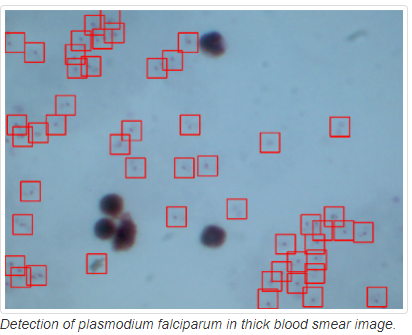
\includegraphics[scale = 0.5]{DP.png} 
	\end{itemize}

	
\end{frame}

\begin{frame}
	\begin{block}{\color{red}{Why is it a data science problem}} \vspace{5pt}\small
		\begin{itemize}
		\item The problem requires a machine to diagnose a disease based on microscope images of bacilli. 
		\item A data science problem is a problem that involves data miing, cleaning and predictive modelling while also providing insights, recommendations and classifications in the process.  
		\end{itemize}
	\end{block}

\begin{block}{\color{red}{Why the solution requires the skills of a data scientist}}\vspace{5pt}\small
	\begin{itemize}
		\item The end result is to have a working model that has been trained to accurately recognise different bacilli.
		
		\item The process involves data gymnastics, and flexibility through complex matrix computations and manipulations.
	\end{itemize}
\end{block}
\end{frame}

\begin{frame}[t]{Role of Maths}
	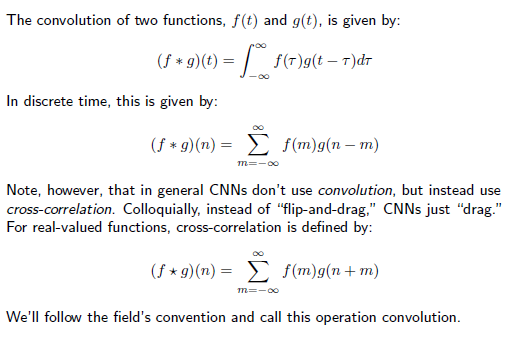
\includegraphics[scale = 0.7]{cnn_math1.png}
\end{frame}

\begin{frame}
	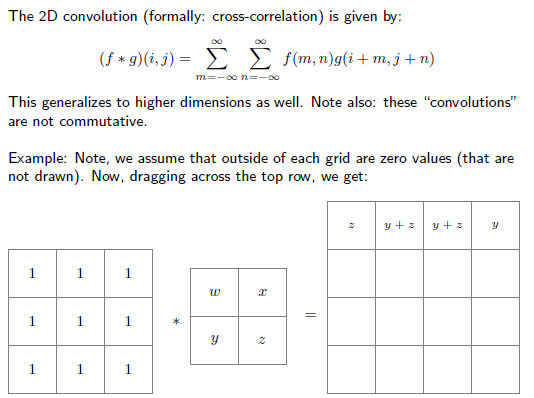
\includegraphics[scale = 0.7]{cnn_math2.png}
\end{frame}

\begin{frame}
	\begin{block}{\color{red}{Convolutional Layer}}
		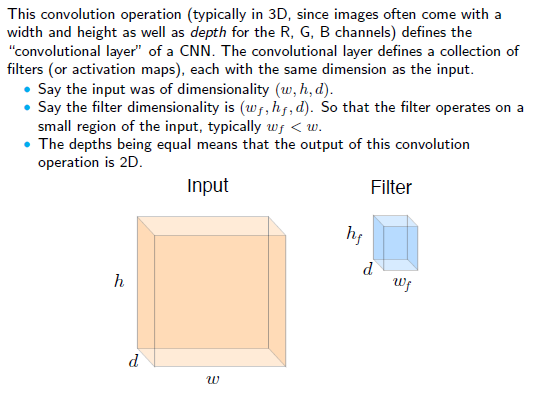
\includegraphics[scale = 0.7]{cnn_math3.png}
	\end{block}
\end{frame}

\begin{frame}[t]{Data Acquisition}
	\begin{block}{\color{red}{Data Sources}}\vspace{5pt}\small
		\begin{itemize}

		\item The data was acquired from \textbf{AI research}: "air.ug/microscopy/" 
		
		\item It is structured since the data consists of images and annotations.
		
		\item The data classifies as big data since each category of disease consists of over 1000 images, each image consisting of thousands of bounding boxes in order to indicate parasites and bacilli.
		
	\end{itemize}
	\end{block}
\end{frame}

\begin{frame}[t]{Data Architecture}
	\begin{block}{}\vspace{2pt}\small
	A one-off customized adapter for any camera and microscope combination is created in order to capture the images from the microscope.\\
	 
	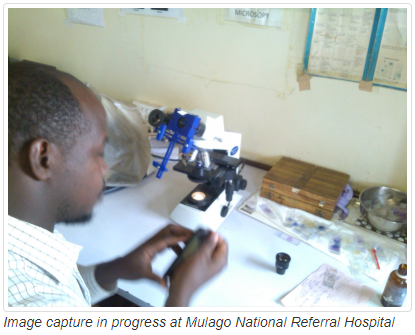
\includegraphics[scale = 0.4]{im_cap.png}
	
	The captured images then preprocessed, before being fed to a model, annotations need to be made. 
\end{block}
\end{frame}

\begin{frame}[t]{Data Analysis}
		\begin{block}{\color{red}{Model Performance}}
		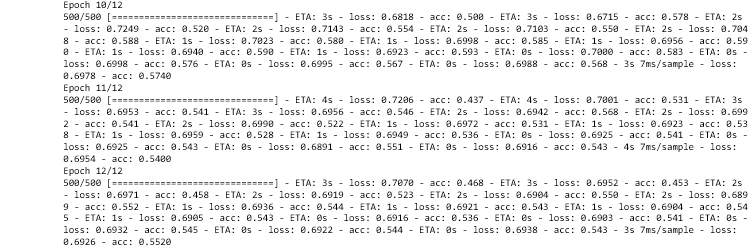
\includegraphics[scale = 0.5]{cnn_model.png}
		\begin{figure}[H]
			\begin{minipage}{\textwidth}
				\centering
				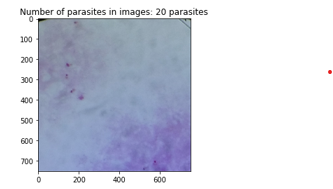
\includegraphics[width=.4\textwidth]{para_in_image.png}
				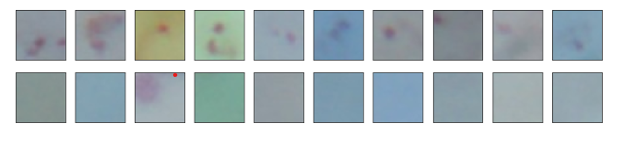
\includegraphics[width=.5\textwidth]{parasites.png}
				\subcaption{Parasites}
				\label{fig:qq_plot}
			\end{minipage}\\[1em]
		\end{figure}
	\end{block}
\end{frame}
	
\end{document}